%! Author = giaco
%! Date = 12/06/2024

\chapter{Results}
\label{sec:results}

\subsection{Main Results}\label{sec:results_1}
In the following empirical evaluation, we used the same methodology and setup adopted for initial experiments. For each game, multiple agents instances are trained using different seeds. For a comprehensive view of agents' performance, the behavior is averaged over different versions. Figure \ref{fig:trainresults} shows the average learning curves of agents during training - the shaded area depicts the standard deviation. To ensure robust evaluation, agents are tested across \texttt{5 random seeds} for \texttt{50 episodes}, specifically: 47695, 32558, 94088, 71782 and 66638. Table \ref{tab:results} reports the averaged results during evaluation of the best agent during training. We address the elephant in the room - Figure \ref{fig:breakouttrain} - in the next section \ref{sec:breakout_study}.

\begin{figure}[ht]
    \centering
    \begin{subfigure}[b]{0.32\textwidth}
        \centering
        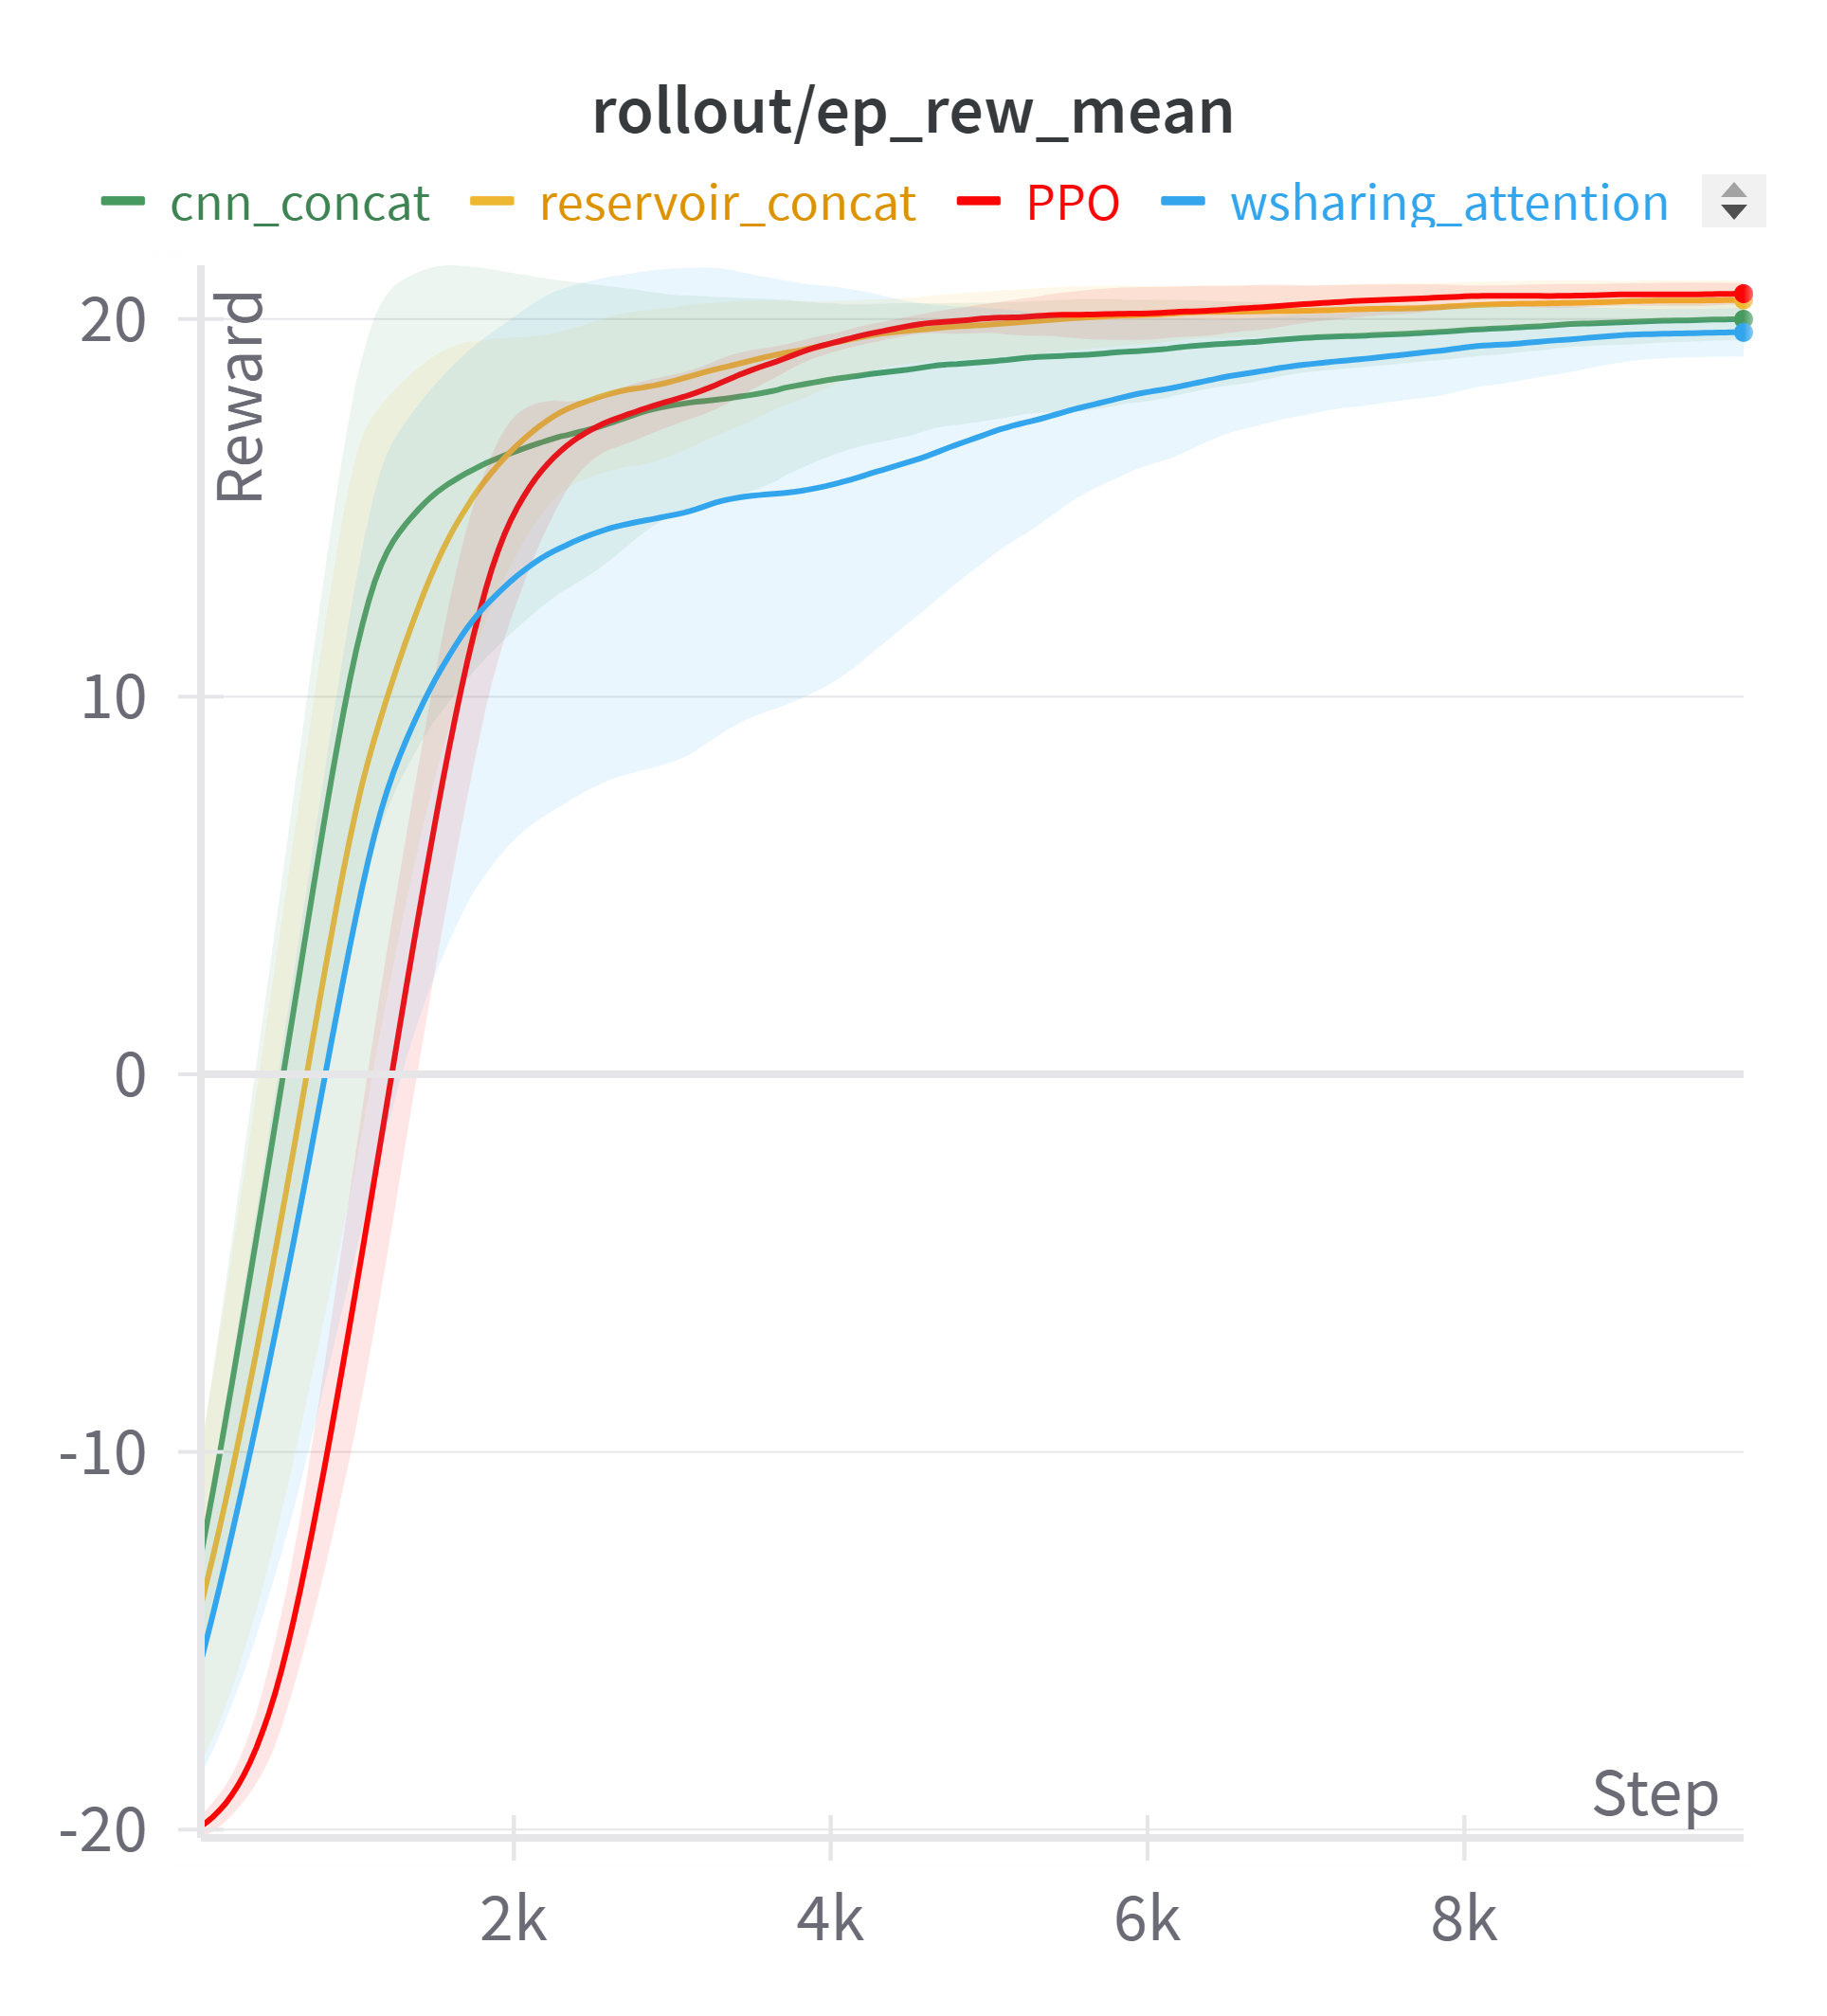
\includegraphics[width=\textwidth]{images/pong_train.png}
        \caption{\texttt{Pong}}
        \label{fig:pongtraining}
    \end{subfigure}
    \hfill
    \begin{subfigure}[b]{0.32\textwidth}
        \centering
        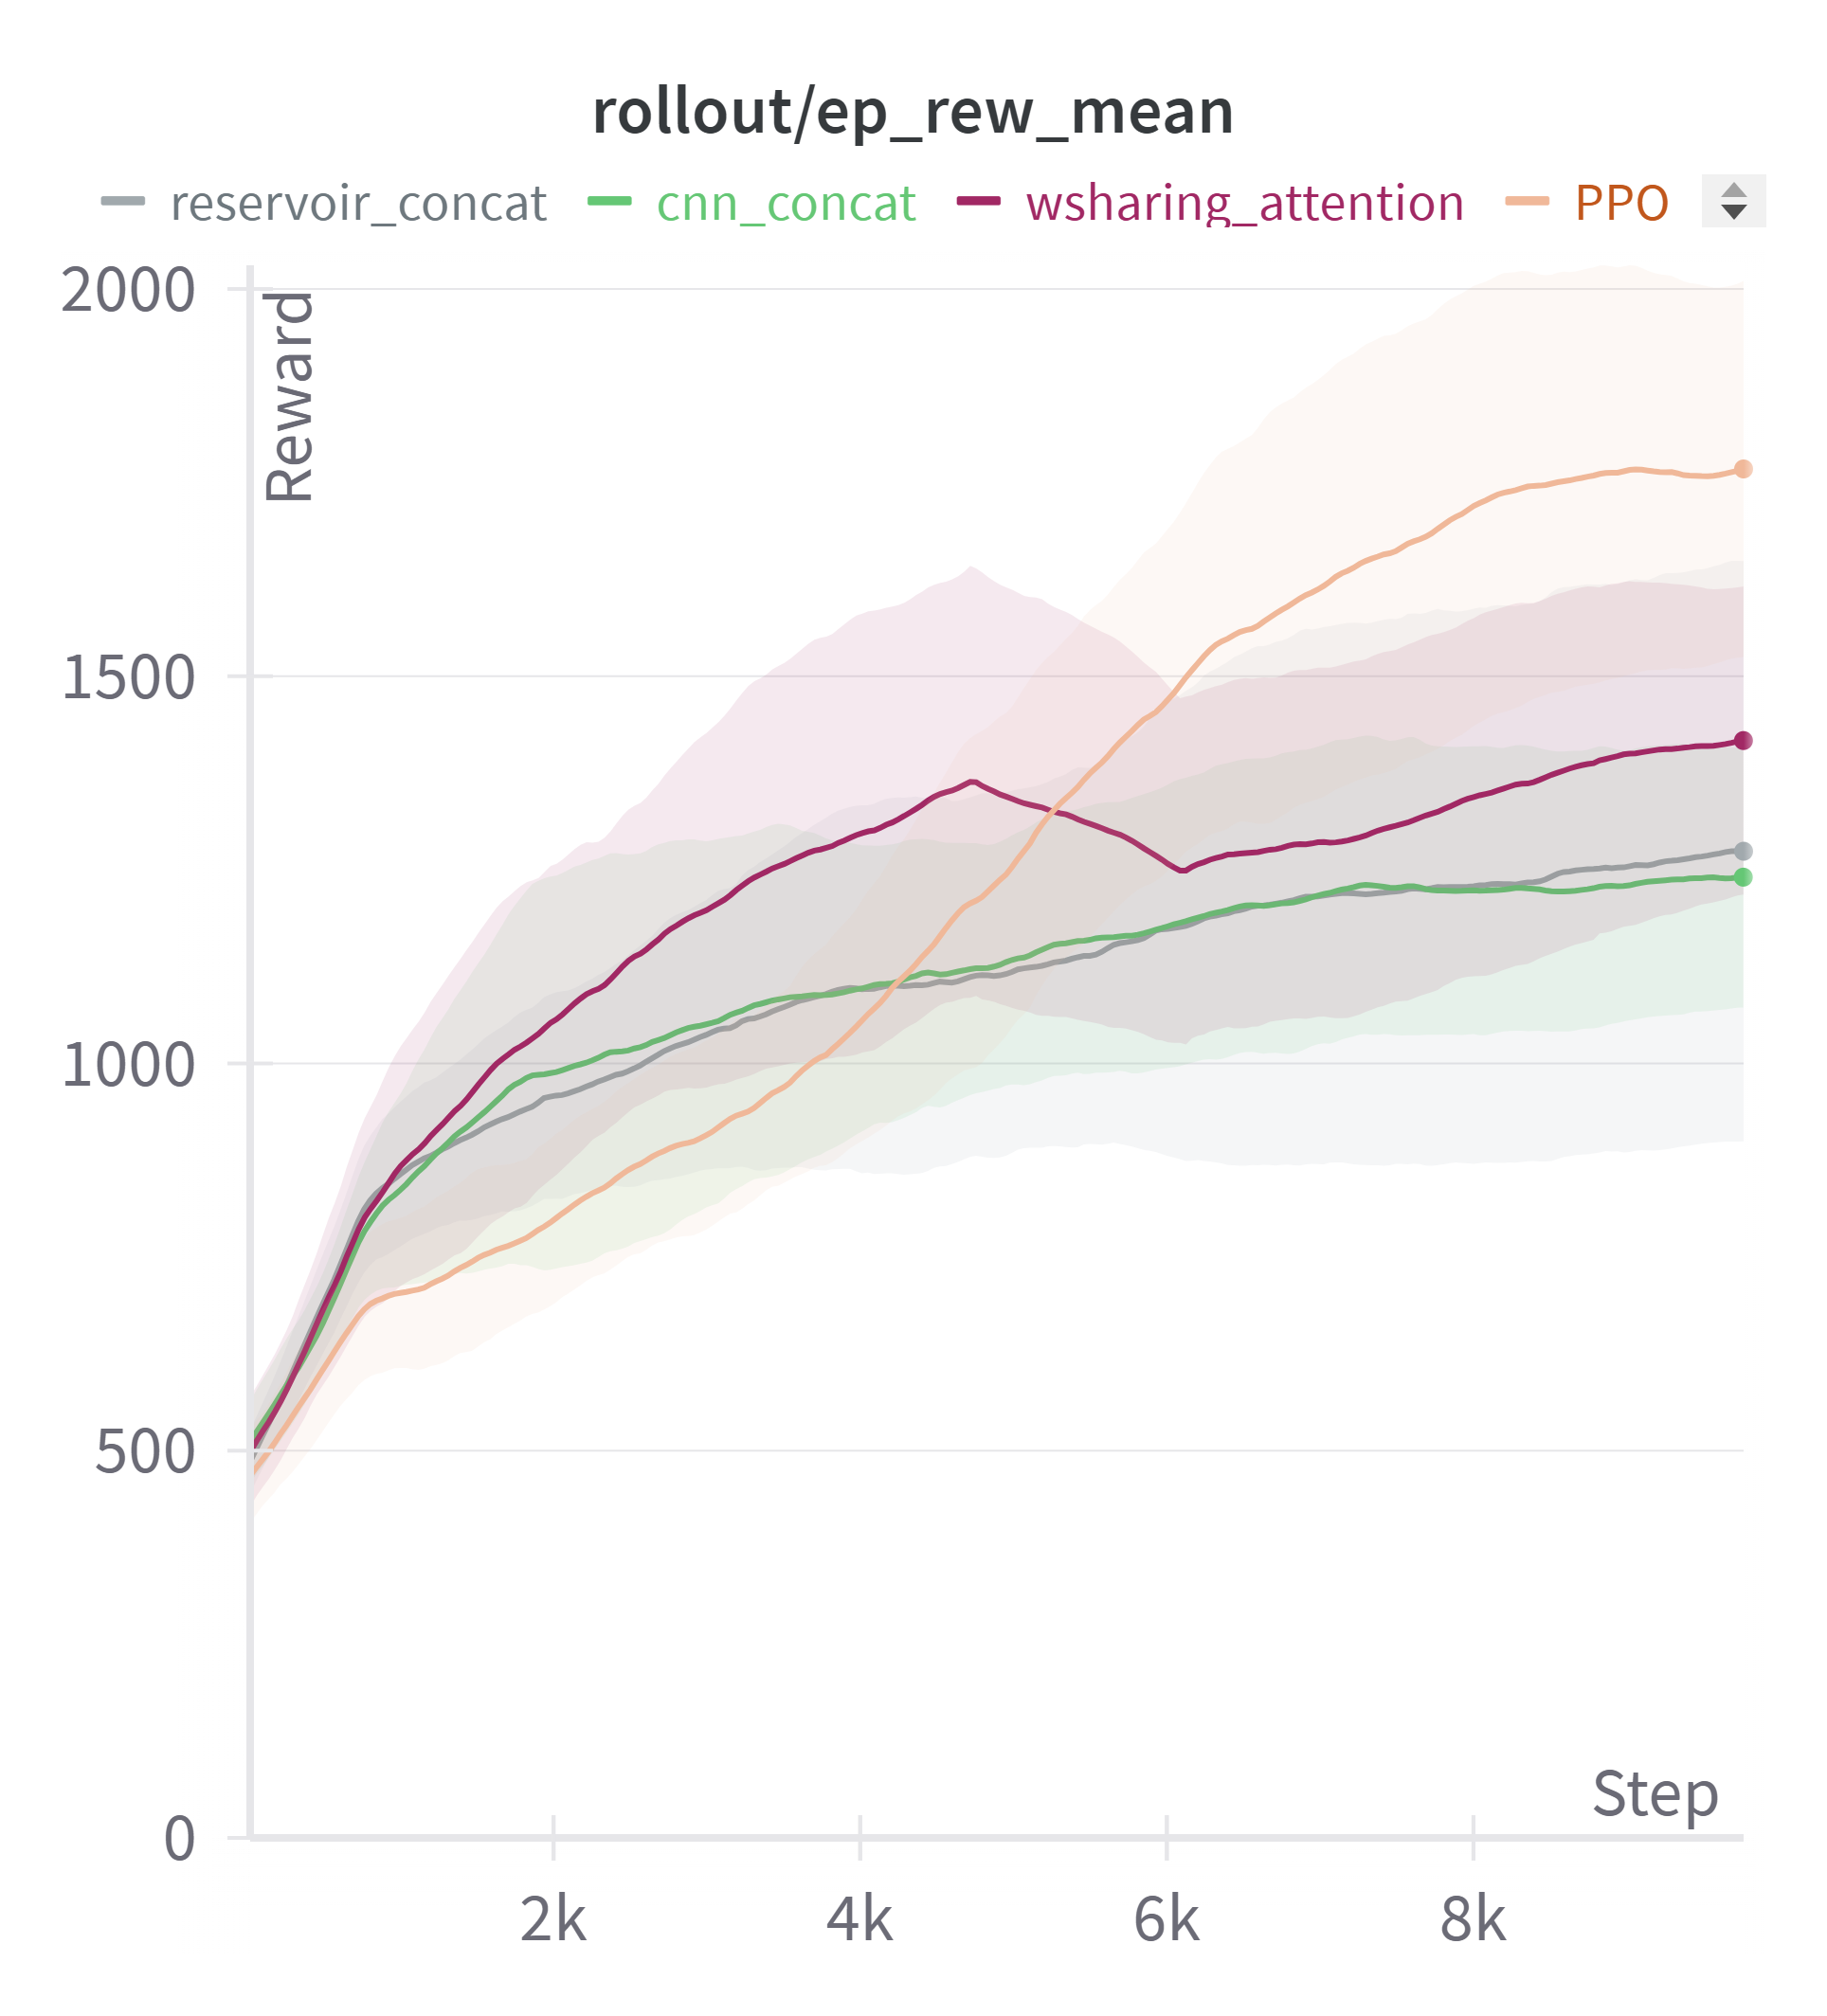
\includegraphics[width=\textwidth]{images/mspacman_train.png}
        \caption{\texttt{Ms.Pacman}}
        \label{fig:mspacmantrain}
    \end{subfigure}
    \hfill
    \begin{subfigure}[b]{0.32\textwidth}
        \centering
        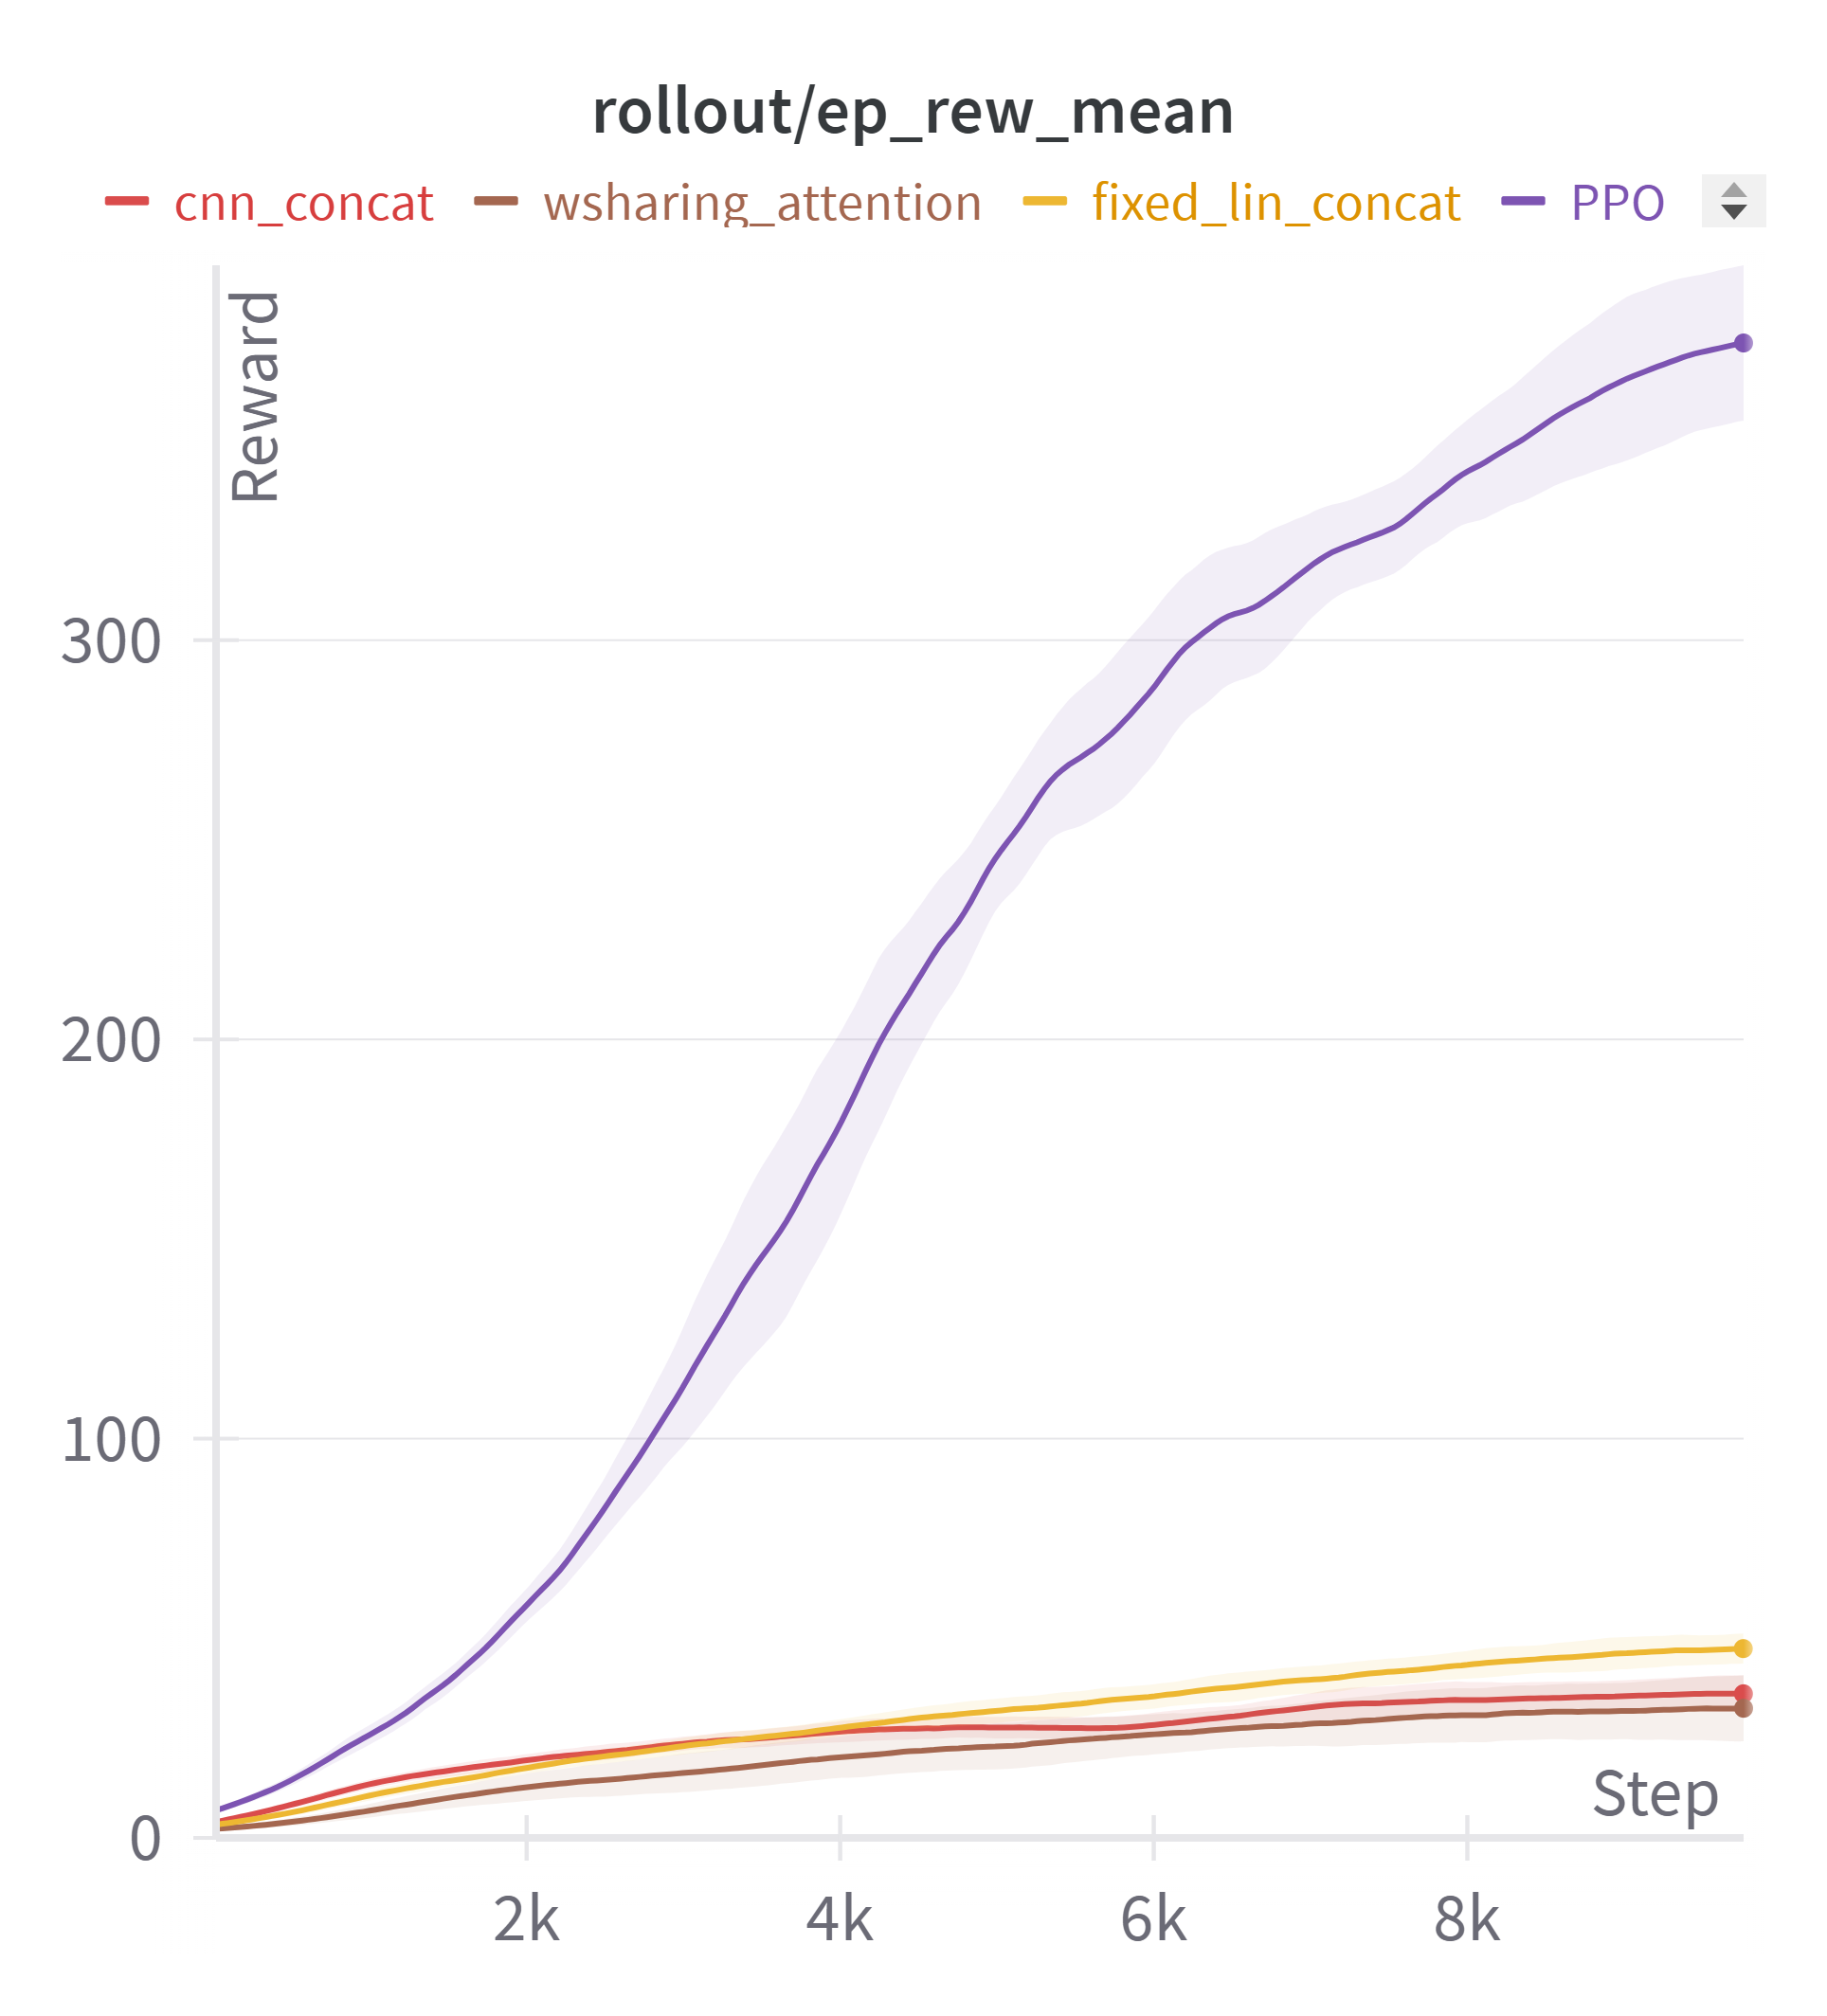
\includegraphics[width=\textwidth]{images/breakout_train.png}
        \caption{\texttt{Breakout}}
        \label{fig:breakouttrain}
    \end{subfigure}
    \caption{Cumulative reward during \texttt{training} of different agents, including WSA, PPO, and other combination modules, on three different Atari games. Each subfigure shows the mean score, with shaded areas indicating the standard deviations, across multiple agents.}
    \label{fig:trainresults}
\end{figure}

Focusing on the first two games, Figures \ref{fig:pongtraining}-\ref{fig:mspacmantrain}, we can see that our approach WSA and other combination modules yield a high reward in the first stages of the training process. This suggests that FMs provide an insightful and comprehensive base of knowledge straight out of the box.
It is important to remember that the results are obtained without conducting any hyperparameter search. Eventually end-to-end PPO catches up and reaches a higher final reward during training. Nevertheless, looking at the evaluation results in Table \ref{tab:results}, WSA matches the maximum reward (\texttt{21}) on \texttt{Pong} and achieves higher score (\texttt{2530}) on \texttt{Ms.Pacman} than PPO (\texttt{2258}). From these results, we can make two important considerations. The first one is the difference between training and evaluation scores. In particular, in \texttt{Ms.Pacman} is more marked, WSA provides a solid generalization for the task, scoring around \texttt{1250} during training compared to \texttt{2530} during evaluation. The second one concerns the difference compared to PPO final score during learning. This behavior is probably related to the well-known phenomenon of underfitting. In fact, with respect to end-to-end solutions, our approach has a limited number of components that are updated during training, in particular the \texttt{Fully-Connected Network} is only one layer. As sanity-check, to ensure agents' performance do not depend on the particular RL algorithm, we also compare WSA effectiveness on \texttt{Ms.Pacman} and \texttt{Breakout} using \texttt{DQN}. Training curves and evaluation scores are reported in Appendix \ref{sec:app-add-exp}.

\subsubsection{Breakout: Out of Distribution Data}\label{sec:breakout_study}
Unexpectedly on \texttt{Breakout}, WSA did not work straightaway. Both in Figure \ref{fig:breakouttrain} and in Table \ref{tab:results}, the performance of WSA is extremely low compared to PPO (\texttt{99 vs 413}).

A first attempt to overcome the problem was to increase the number of parameters of the model, adding more expressive power to the network learning the policy. We increased the size of the \texttt{Fully-Connected Network} to three linear layers of size 1024, 512, and 256 respectively and use ReLU as activation function. Figure \ref{fig:breakout_policy} and Table \ref{tab:results} - referenced as \texttt{(P)} - report the results for this experiment. With respect to the default scenario, there is an improvement in performance, but WSA is still far from PPO (\texttt{156 vs 413)}.

\begin{figure}[ht]
    \centering
    \begin{subfigure}[b]{0.32\textwidth}
        \centering
        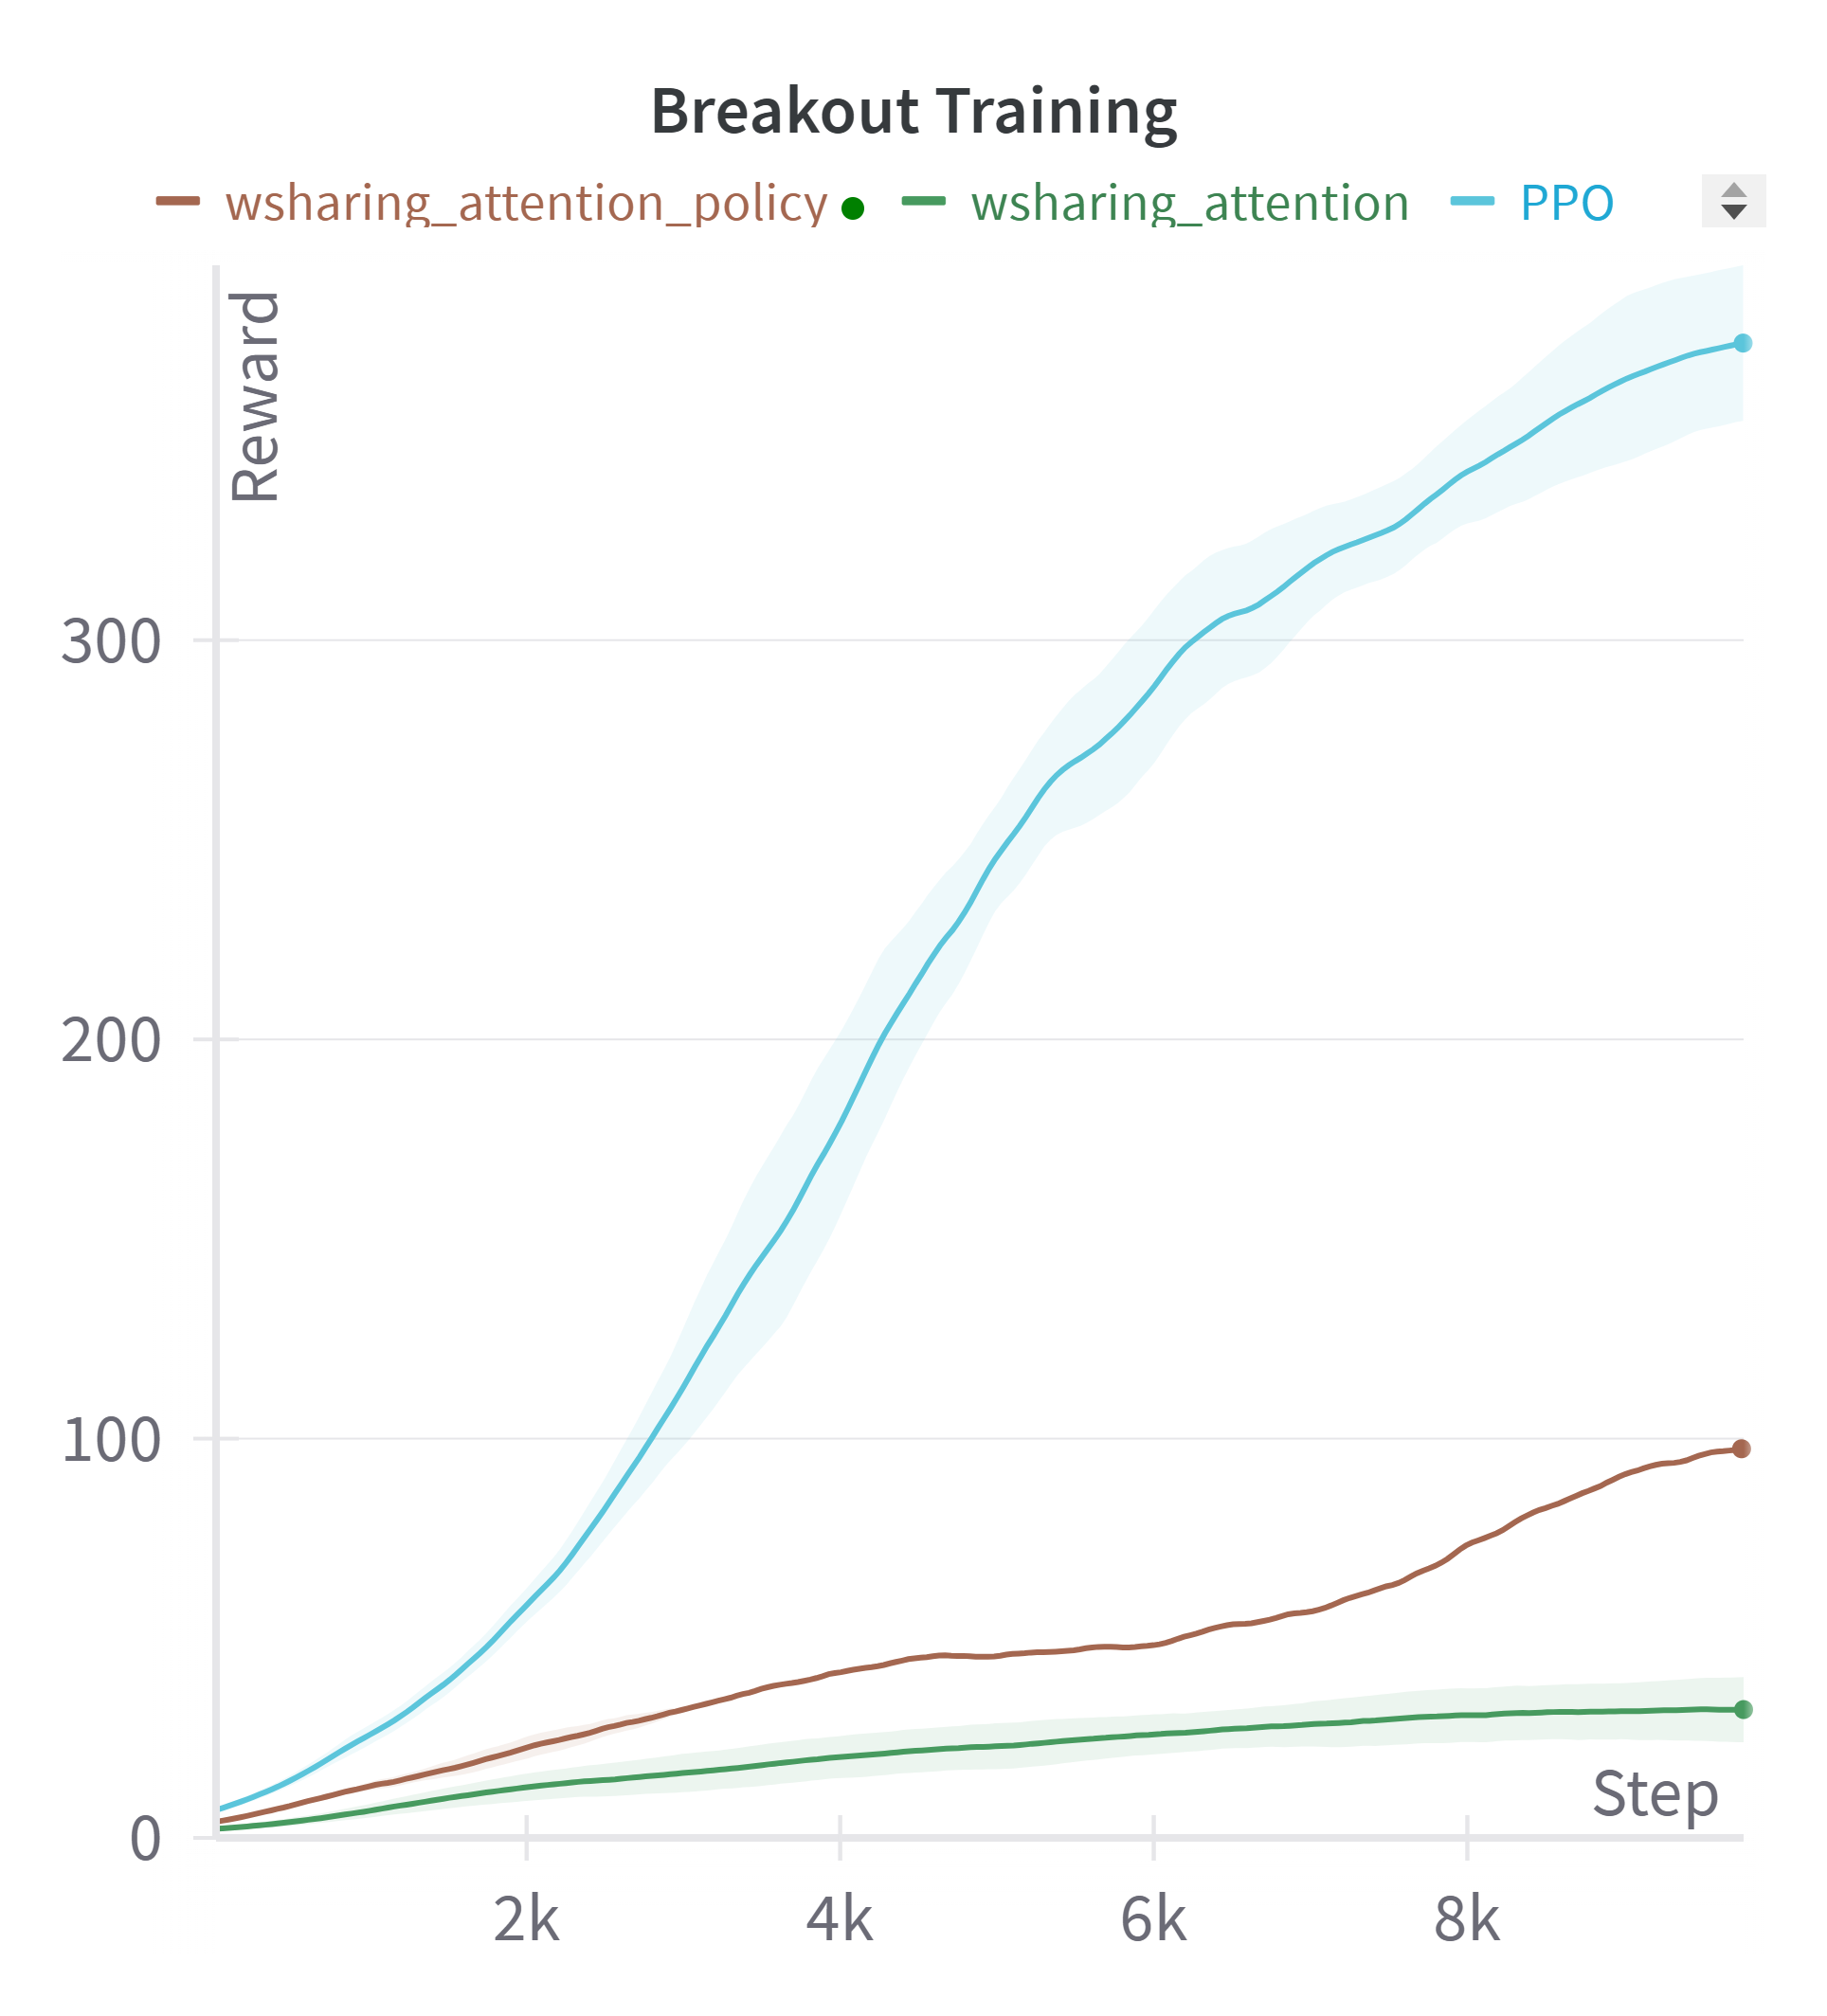
\includegraphics[width=\textwidth]{images/breakout_policy.png}
        \caption{Increasing MLP size}
        \label{fig:breakout_policy}
    \end{subfigure}
    \hfill
    \begin{subfigure}[b]{0.32\textwidth}
        \centering
        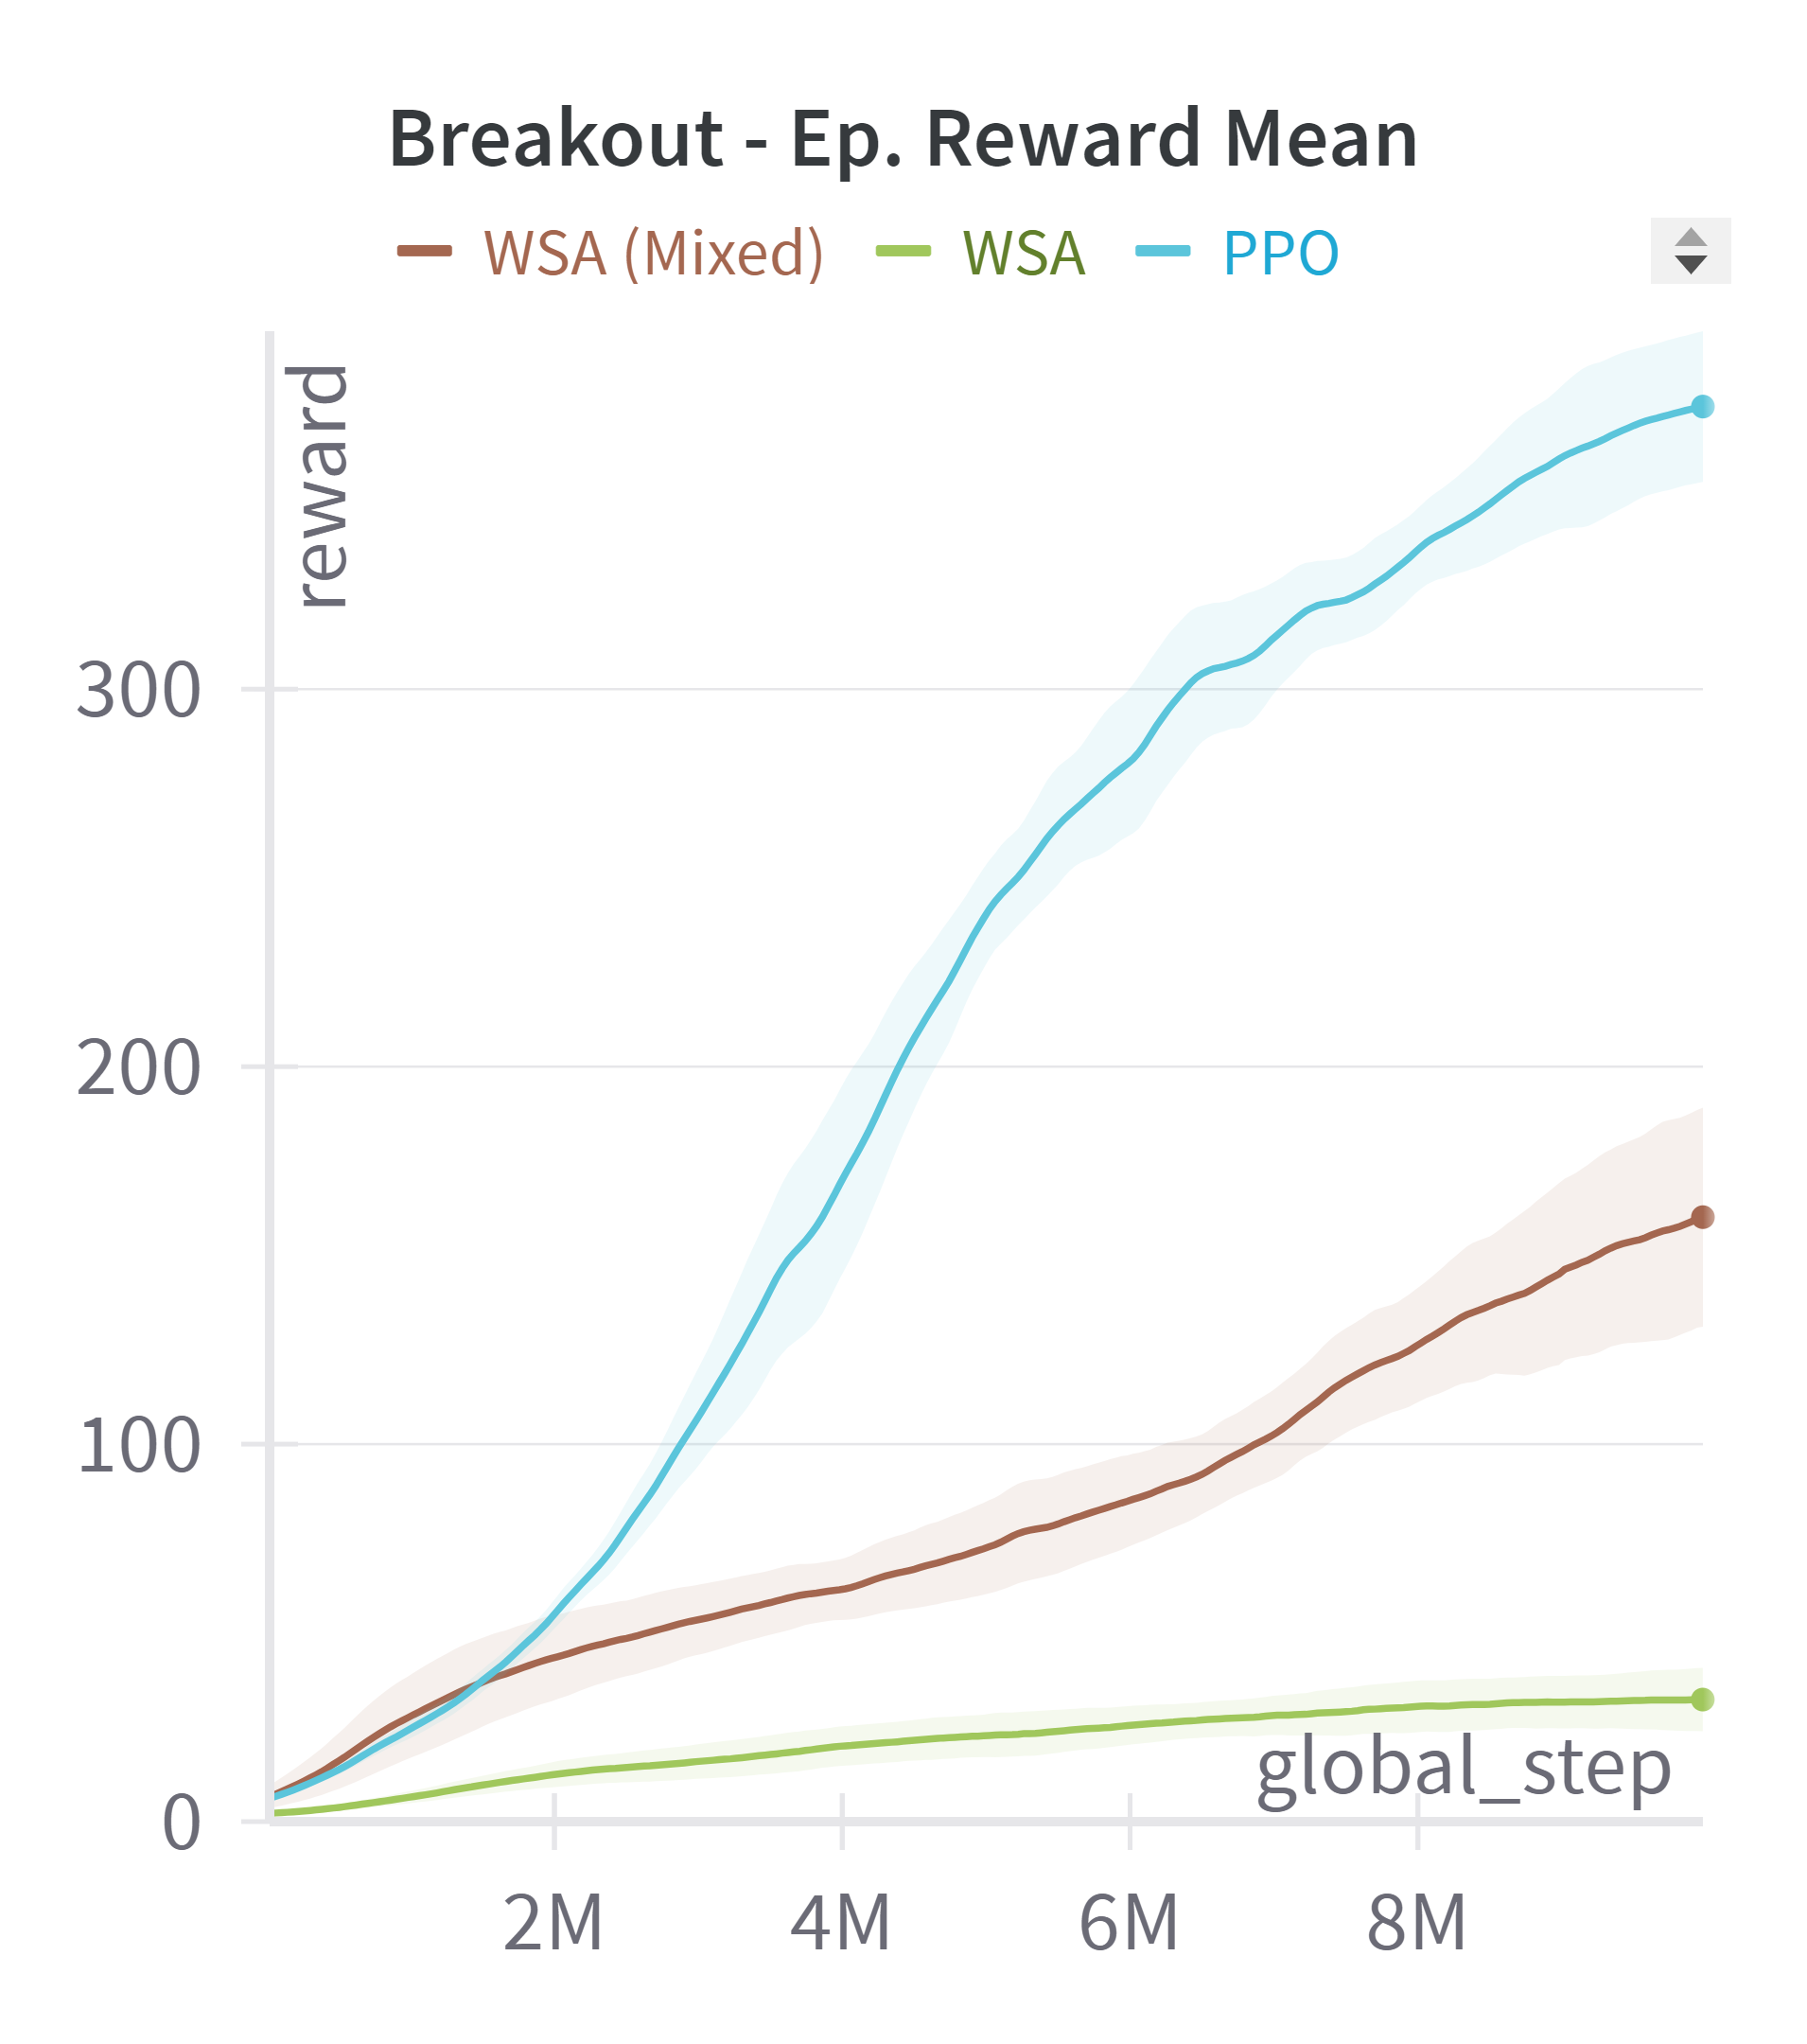
\includegraphics[width=\textwidth]{images/breakout_expert.png}
        \caption{Using Mixed Data}
        \label{fig:breakout_expert}
    \end{subfigure}
    \hfill
    \begin{subfigure}[b]{0.32\textwidth}
        \centering
        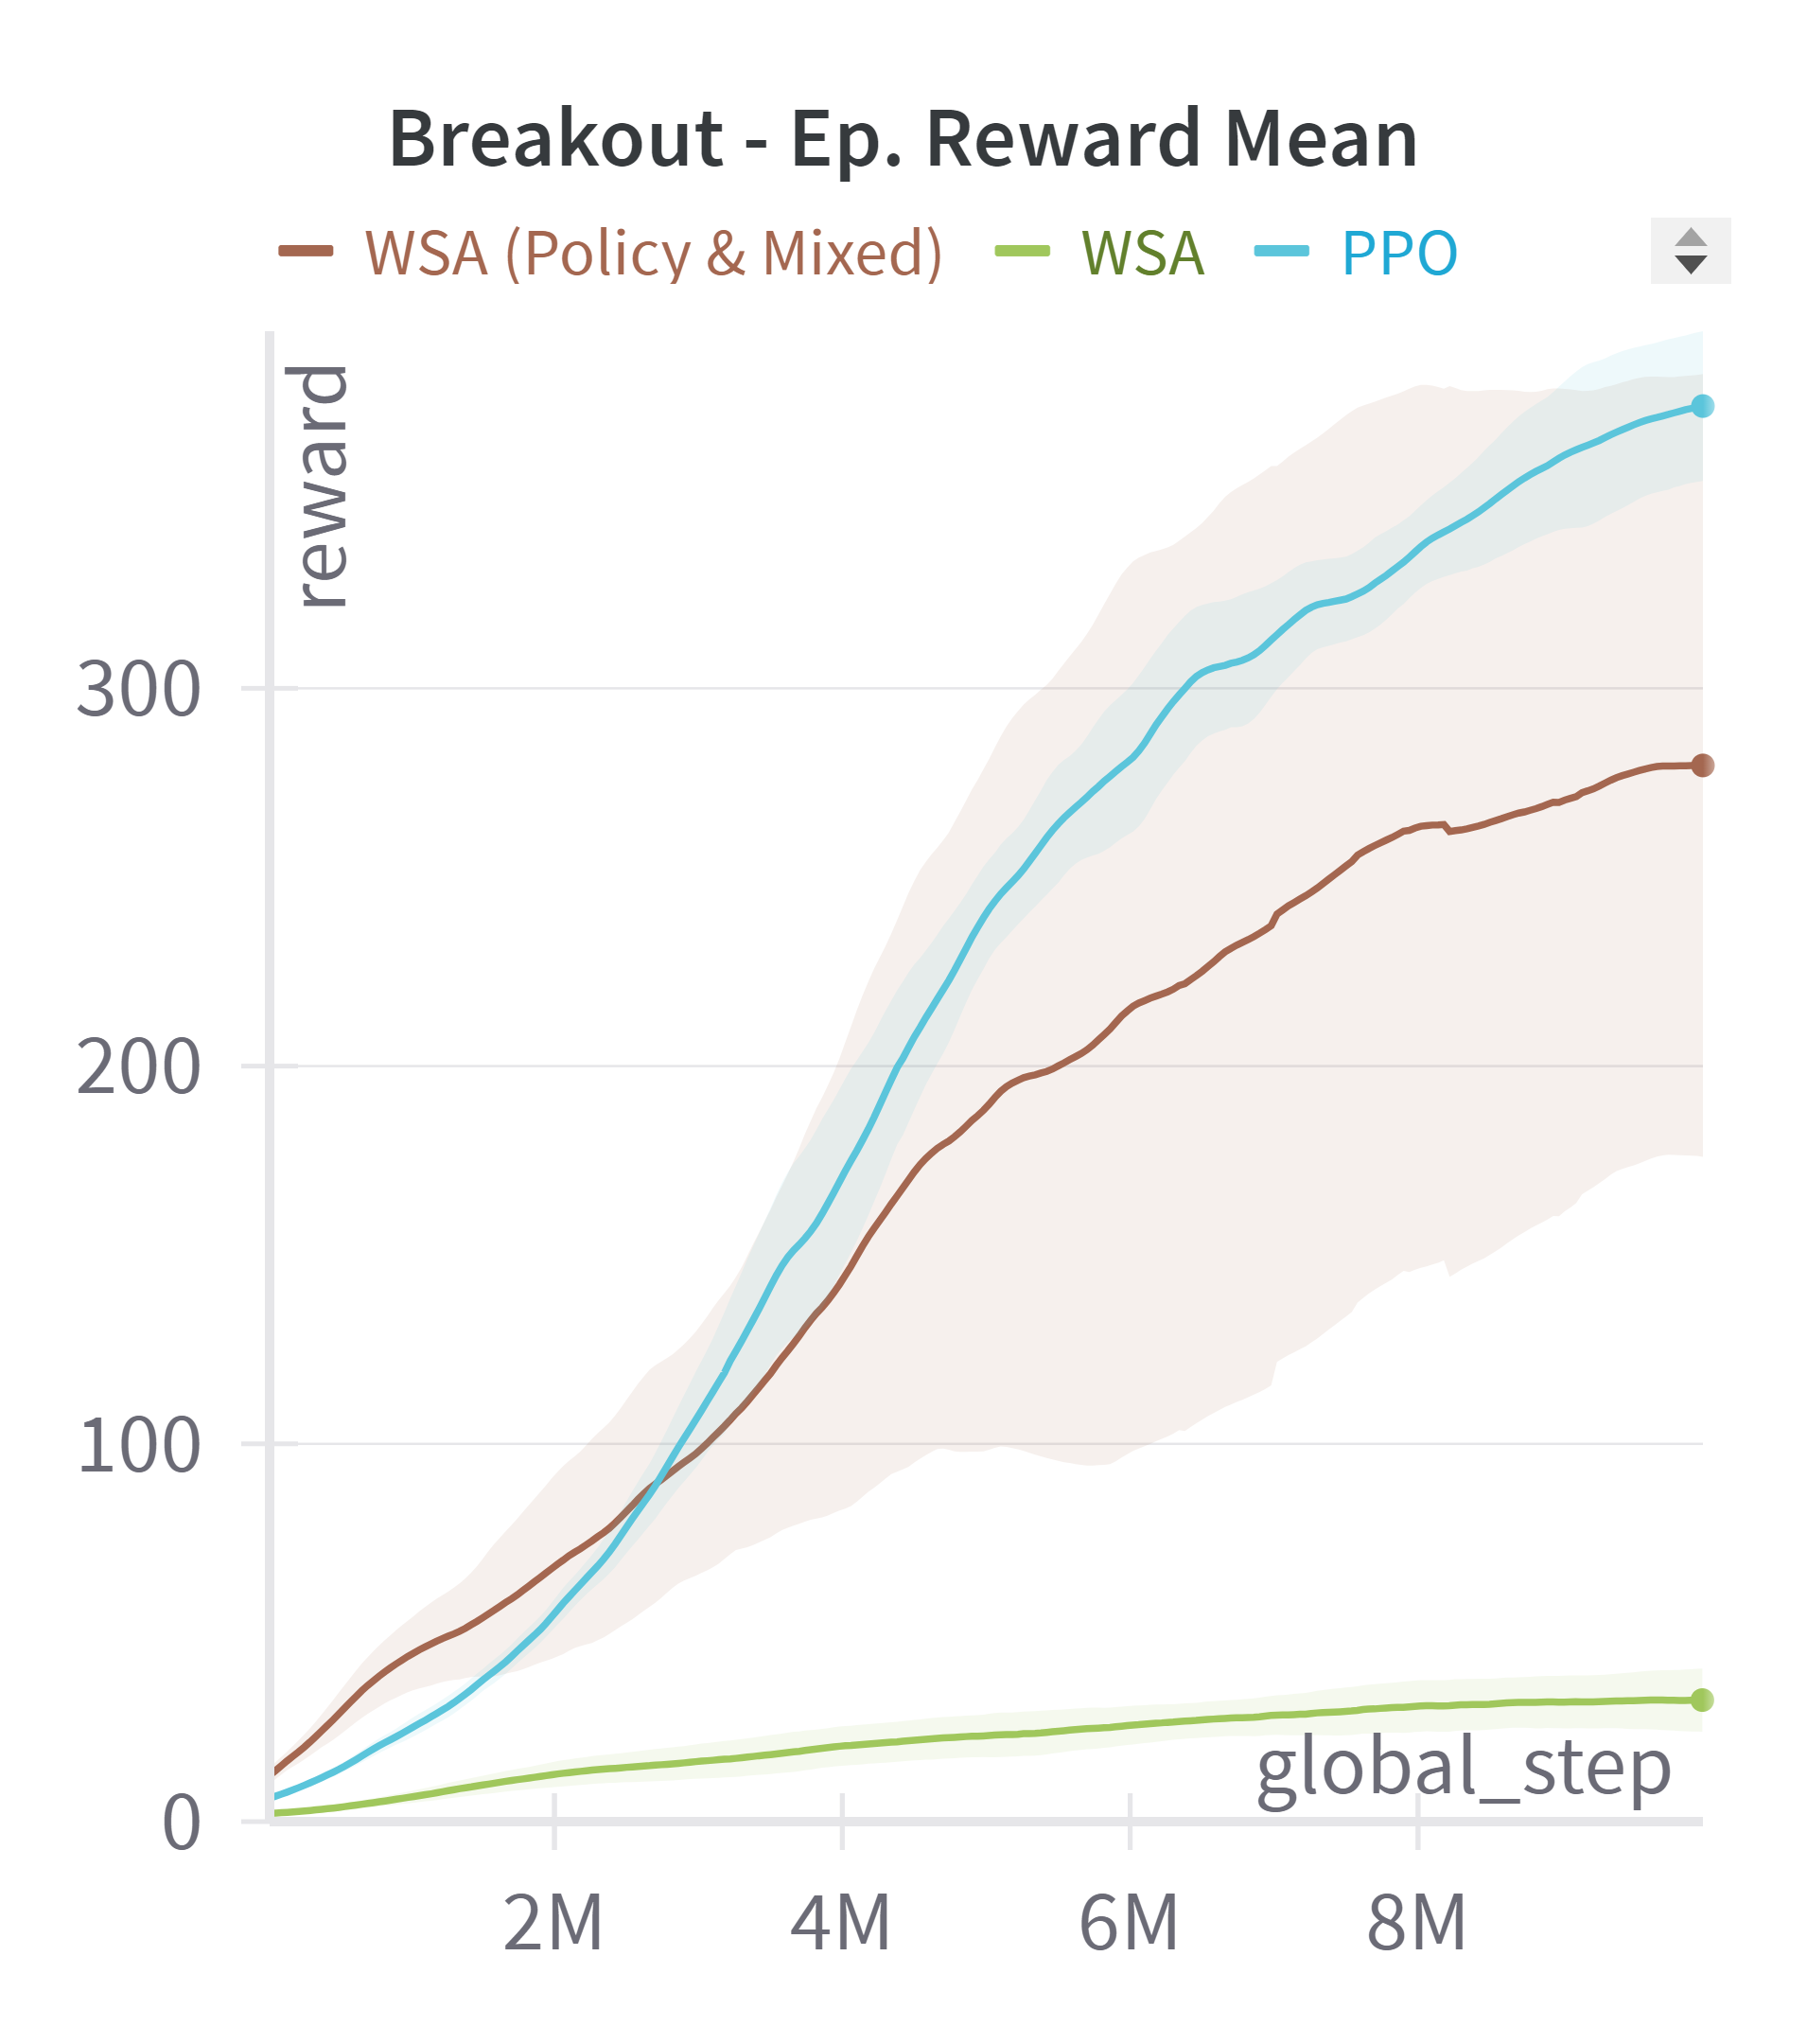
\includegraphics[width=\textwidth]{images/breakout_policy_mixed.png}
        \caption{Mixed Data + Increased MLP}
        \label{fig:breakout_expert_policy}
    \end{subfigure}
    \caption{Performance comparison of WSA with PPO across various strategies on \texttt{Breakout}. Each subfigure displays the average score with the standard deviation shaded. They report the different experiments to improve the performance of WSA: (\ref{fig:breakout_policy}) increasing the size of the \texttt{Fully-Connected Network} on performance, (\ref{fig:breakout_expert}) pre-training the models using random data and expert data, and (\ref{fig:breakout_expert_policy}) combining the effect of increased \texttt{Fully-Connected Network} and expert data during pre-training.}
    \label{fig:breakout_study}
\end{figure}

Before moving on to the next set of experiments, which close the gap between PPO and WSA, we address a key challenge when using pre-trained models in RL. Unlike \texttt{Pong} and \texttt{Ms.Pacman}, where the game screen remains relatively stable, \texttt{Breakout} dynamically evolves as more blocks are removed with score progression. This poses a \textbf{distributional shift} problem between training and test data. Our initial training data, collected from random agents, lacks late game scenarios with few blocks remaining, leading to limitations in FMs performance during evaluation. To tackle the problem and show the consequences of a limited training dataset, we gather new datasets from both random and expert agents to encompass early and late game scenarios.

We retrain all the FMs and RL agents - using a single layer \texttt{Fully-Connected Network}. Significant improvements are observed, as shown in Figure \ref{fig:breakout_expert} and Table \ref{tab:results}, using (\texttt{M}). Notably, WSA demonstrates a substantial increase in the agent's final score (\texttt{156 $\rightarrow$ 345}), approaching PPO performance, and echoing the trends analyzed in Section \ref{sec:results_1} for the other two games. To complete the set of experiments, we also test the combination of the previous configuration. Increased \texttt{Fully-Connected Network} and Mixed datasets (Figure \ref{fig:breakout_expert_policy}, \texttt{PM}) yields the best performing configuration of WSA with slightly lower but competitive score to PPO (\texttt{387 vs 413}). Additionally, Appendix \ref{sec:app-add-exp} reports the same analysis for the other combination modules presented in Figure \ref{fig:breakouttrain}.

Lastly, Figure \ref{fig:inter} illustrates the enhanced \texttt{explainability} provided by WSA. By examining the current frames and the corresponding weights allocated by the shared component to each pre-trained model, one can appreciate agents' decision-making process. The visualization reveals how various FMs are leveraged in distinct contexts, shedding light on agents' dynamic adaptation of its prior knowledge.

\begin{table}[ht]
\begin{minipage}[b]{0.49\linewidth}
\centering
    \begin{tabular}[b]{lll}
                \multicolumn{1}{l}{Environment}  &\multicolumn{1}{l}{\bf Agent} &\multicolumn{1}{l}{\bf Reward} \\
                \hline \\
                \multirow{5}{*}{\texttt{Pong}} & \textbf{CNN} & \textbf{21 $\pm$ 0.00} \\
                                      & RES & 20.85 $\pm$ 0.29 \\
                                      & \textbf{WSA} & \textbf{21 $\pm$ 0.00} \\
                                      & \textbf{PPO} & \textbf{21 $\pm$ 0.00}\\

                                      \hline \\
                \multirow{5}{*}{\texttt{Ms.Pacman}} & CNN & 1801.30 $\pm$ 20.95 \\
                                      & RES & 1369.27 $\pm$ 565.23 \\
                                      &\textbf{WSA} & \textbf{2530.20 $\pm$ 23.09} \\
                                      & \underline{PPO} & \underline{2258.40 $\pm$ 1.42}\\
                                      \hline \\

                \multirow{7}{*}{\texttt{Breakout}}
                                      & CNN & 65.98 $\pm$ 1.62 \\
                                      & FIX & 87.17 $\pm$ 6.87 \\
                                      & WSA & 99.58 $\pm$ 6.66 \\
                                      & WSA (P) & 156.17 $\pm$ 3.59 \\
                                      & WSA (M) & 345.52 $\pm$ 6.47 \\
                                      & \underline{WSA} (PM)& \underline{387.15 $\pm$ 0.43} \\
                                      & \textbf{PPO} & \textbf{413.51 $\pm$ 1.10}\\
    \end{tabular}
    \caption{Performance during \texttt{evaluation} averaged across 5 different seeds.}
    \label{tab:results}
\end{minipage}\hfill
\begin{minipage}[b]{0.49\linewidth}
\centering
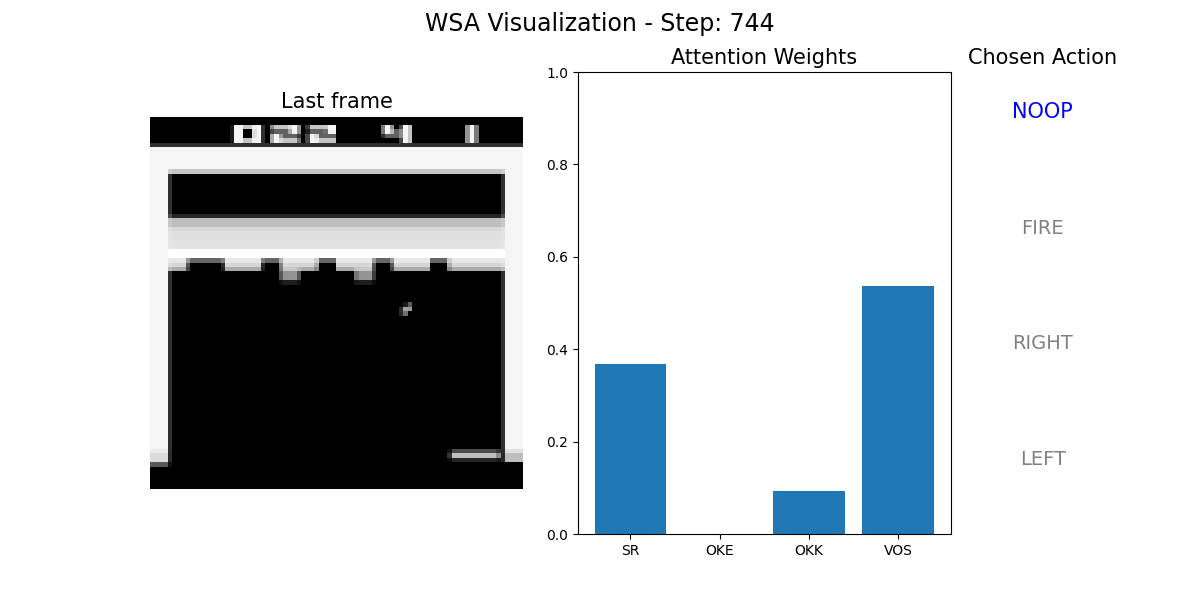
\includegraphics[width=\textwidth]{images/744.png}
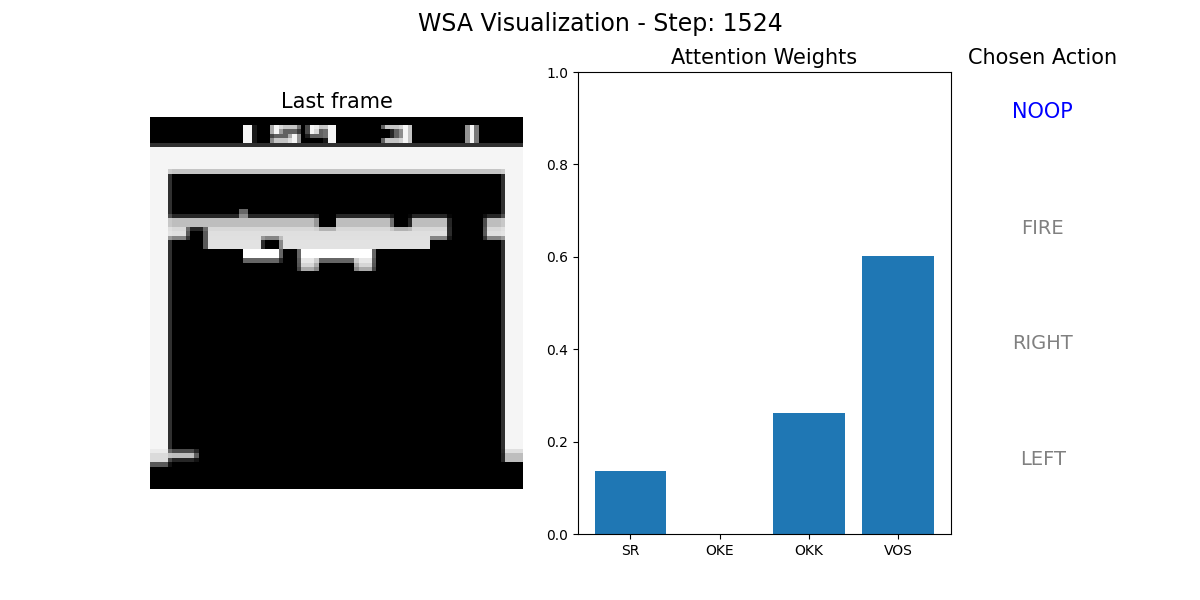
\includegraphics[width=\textwidth]{images/1524.png}
\captionof{figure}{Analyzing WSA explainability across different frames, showcasing the weights assigned to different FMs.}
\label{fig:inter}
\end{minipage}
\end{table}